\documentclass{article}

\usepackage{enumitem}
\usepackage{graphicx}

\setlength{\parindent}{0em}

\graphicspath{ {./images/} }

\newcommand\setItemnumber[1]{\setcounter{enumi}{\numexpr#1-1\relax}}

\title{ \LARGE Web  Applications and Services\\
 \Large Assignment 1: Online Payment System}
    
\author{University of Sussex \\
	Candidate Number: 164574}
	
\date{}

\begin{document}

\maketitle

\newpage

\tableofcontents

\newpage

Note: Netbeans ignored changes for context root and marks will not be deducted as discussed on discord.

\section{Design}

The model-view-controller software pattern is commonly used for developing user interfaces, which divides each section of the program into three distinct interconnected components. These three components are the model, the view and the controller. The model is the central component which usually reflects real-world objects and is used to store raw data. The view is a representation of the model to the user and the controller acts as a liaison between the model and the view, accepting input, updating the model and producing output for the view \cite{deacon2009model}.

\begin{figure}[h!]
  \centering
  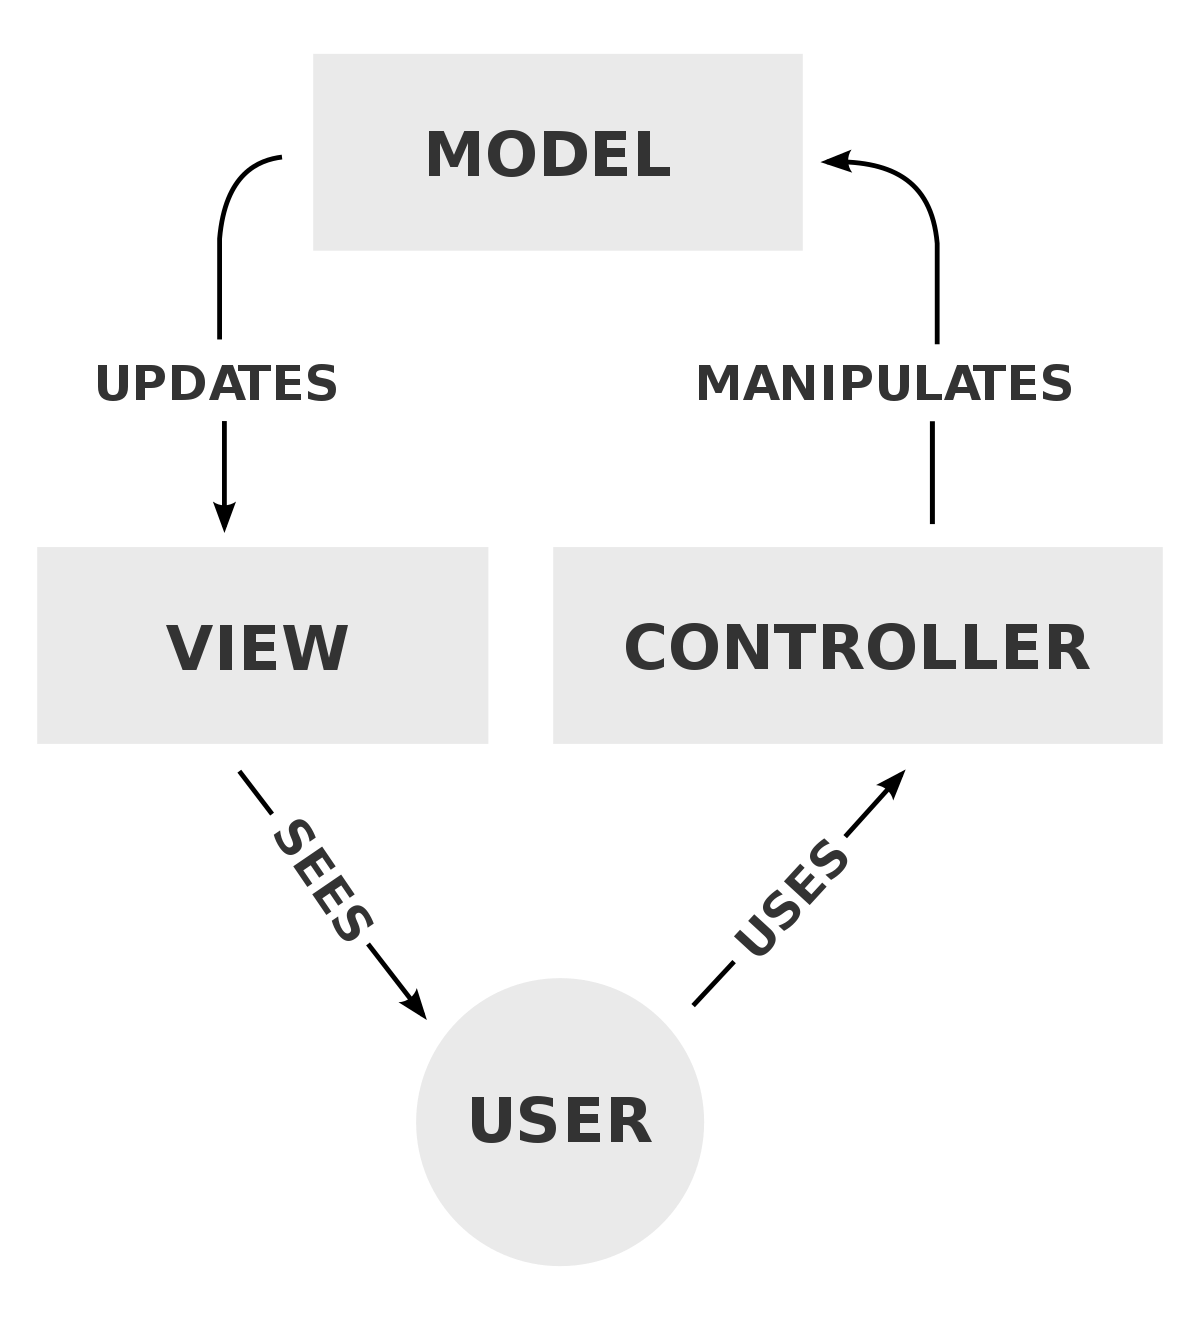
\includegraphics[width=0.4\textwidth]{images/mvc.png}
  \caption{MVC Design Pattern \cite{mvc}}
\end{figure}

The design of the web application fits with the 3-tier architectural model. The model component in the web application are the entities and Enterprise Java Beans. An entity is a lightweight persistence domain object which represents a table in a relational database \cite{entites}, modelling and encapsulating the raw data of the web application. This can be seen in the design of the web application through the entity classes, which model the real-world objects. The handling of the entities are Enterprise Java Beans. Enterprise Java Beans represent the business functionality and the management of the data represented by entities. \\

The view component is handled by Web Pages which include xhtml files and JavaServer Faces components to build the view. These web pages include backing beans which render data from the model to the user of the web application. \\

The controller is responsible for managing and processing input and requests. The controller can be demonstrated in the design of the web application through the use of JavaServer Faces managed beans. These are Java Beans that are managed by the JSF framework \cite{jsfmanagedbeans}. All user interactions with the web application are handled by a front-end 'Faces' servlet which acts as the controller \cite{whatisjsf}. This can be seen in the web applications jsf package which contains managed beans which are responsible for producing output for the view and interacting with EJB's to update the models.

\begin{figure}[h!]
  \centering
  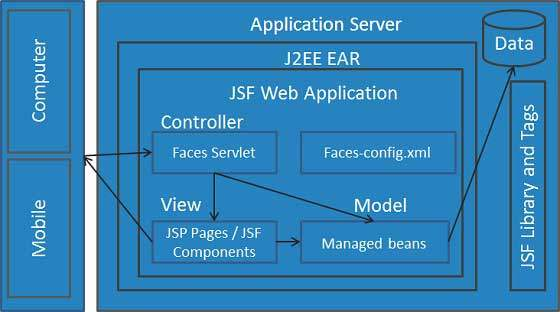
\includegraphics[width=0.7\textwidth]{images/jsfarchitectute.jpg}
  \caption{JSF Architecture \cite{jsf}}
\end{figure}

\newpage

\section{Security}

Security is vital for any multi-user web application to prevent unauthorised entities from compromising the integrity of the system. An authentication realm is a scope over which an application server defines and enforces a common security policy. The chosen method for securing the application is form-based authentication using a JDBCRealm which contains a collection of users who are assigned to groups. As the application uses a JDBCRealm for user authentication it allows the application to dynamically register new users and store their credentials to a relational database system and retrieve user credentials from the database. This approach has the advantage that it provides a place to securely store and retrieve user information. JDBCRealms also provide the functionality to assign security roles to users or groups through the application server-specific deployment descriptor \cite{JDBC}. Users are assigned to groups during the user creation process and this is more efficient that mapping security roles to individual users. \\

The strengths of the mapping of security roles to groups is the implementation of declarative security to restrict access to web pages to non-authorised user and access to EJB methods. Declarative security expresses an application component’s security requirements by using either deployment descriptors or annotations \cite{security}. Annotations are used throughout the web application to allow user roles to access certain EJB methods and web pages through security constraints. The advantage of this method is that after a user has been authenticated, the user is permitted to perform the actions related to their user group which aligns with the logic of the system and denies attempts of accessing data from non-authorised users. A weakness of this approach is that using this type of validation makes the system prone to password based attacks. This is a common issue across all web applications and the way to make the system more secure against these attacks are a strong password policy and strong salt and hashing algorithms. \\

HTTPS is enabled to preserve the integrity of the system. The strength of using this over HTTP is that HTTPS uses TLS(SSL) to encrypt normal HTTP requests and responses \cite{https}.

\begin{figure}[h!]
  \centering
  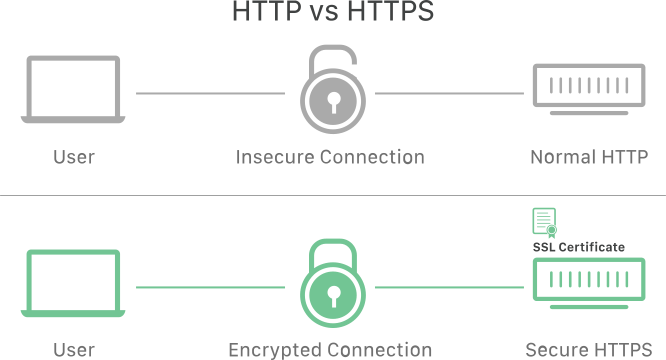
\includegraphics[width=0.5\textwidth]{images/http-vs-https (1).png}
  \caption{HTTP vs HTTPS \cite{https}}
\end{figure}

\newpage

\section{Extended design to deal with single point of failure}

A single point of failure is a part of a system that, if it fails, will stop the entire system from working. Single point of failures can be divided into three categories \cite{SPOF}:
\begin{itemize}
    \item Hardware failures, for example, server crashes, network failures, power failures, or disk drive crashes
    \item Software failures
    \item Database corruption
\end{itemize}
A way to deal with a single point of failure for hardware failures is to allow for multiple deployments onto multiple machines through clustering. This mitigates the single point of failure as if there is a hardware failure or the sever crashes, the application is can still operate. \\

Extending the application design to deal with software failures involves restarting the sever when there is a failure. Software failures can range for many different reasons, including issues with application specific code. To mitigate risk of a single point of failure at the software level is intricate, the best practices are to restart the server if the system becomes redundant and identify and fix the single point of failure.

\newpage

\section{Concurrency}

Concurrency is the concept of executing two or more tasks in parallel \cite{concurrency}. This is vital for a multi-user system with users accessing functionality and data. Singleton session beans are designed for concurrent access, where many clients may need to access a single instance of a session bean at the same time \cite{concurrencybean}. This allows for multiple users to access the functionality of the system. \\

Since the functionality of the system involves user transactions, issues arise around concurrency control. A transaction  is a set of operations on objects to be performed as an indivisible unit by the servers managing those objects. Transactions follows the ACID properties, which stands for Atmoic, Consistent, Isolated and Durable. The use of transactions can lead to issues regarding concurrency control, where different transactions access different functionality and data can cause lack of consistency. The web application uses container managed transactions, where the EJB container manages the transaction states \cite{transactions}. Typically, the container begins a transaction immediately before an enterprise bean method starts and commits the transaction just before the method exits \cite{transactions}. Each method can be associated with a single transaction \cite{transactions}. The web application uses the Required Transaction attribute, which is the implicit transaction attribute for all enterprise beans. \\

Another method of dealing with concurrency is the entity manager flush method. When the method is called, all queries with the associated entity are executed in the database. This prevents issues with concurrency and deadlock as two transactions cannot retrieve and manipulate data in the database at the same time.\\

The system could be extended to deal with concurrent users accessing functionality and data by implementing an automatic roll back of the transaction if a system exception is thrown. Another way the system could be extended could be JPA second level (L2) caching. The advantages of L2 caching include avoiding database access for already loaded entities and faster for reading frequently accessed unmodified entities.

\newpage

\bibliography{references}
\bibliographystyle{ieeetr}
\newpage

\end{document}
